\documentclass[11pt]{article}

\usepackage[spanish]{babel}
\decimalpoint
\addto\captionsspanish{\def\tablename{Tabla}}
\usepackage[T1]{fontenc}
\usepackage[margin=1in]{geometry}
\usepackage{amsmath, amssymb, amsfonts}
\usepackage{booktabs}
\usepackage{enumitem}
\usepackage{tcolorbox}
\usepackage[hidelinks]{hyperref}
\usepackage{listings}
\usepackage{xcolor}
\usepackage[skip={0.6em plus 0.2em}]{parskip}
\usepackage{csquotes}
\usepackage{adjustbox}
\usepackage{array,tabularx}
\usepackage{pgfplots}
\usepackage{graphicx}
\usepackage{float}
\usepackage{needspace}
\usepackage[backend=biber,style=numeric,sorting=none]{biblatex}
\addbibresource{referencias.bib}

\newcolumntype{Y}{>{\raggedright\arraybackslash}X}
\emergencystretch=3em
\usetikzlibrary{arrows.meta}
\pgfplotsset{compat=1.18}

\lstset{
  language=Python,
  basicstyle=\ttfamily\footnotesize,
  breaklines=true,
  columns=flexible,
  keepspaces=true,
  commentstyle=\color{gray}\itshape,
  keywordstyle=\color{blue!70!black}\bfseries,
  stringstyle=\color{green!40!black},
  frame=L,
  xleftmargin=2em,
  showstringspaces=false,
  tabsize=4
}

\graphicspath{{figures/}}

% Pendiente del autor (naranja), borrador de interpretación (azul) y material generado por IA (morado)
\newtcolorbox{pendiente}{colback=orange!8,colframe=orange!70!black,title={Por completar},fonttitle=\bfseries\small,boxrule=0.6pt,left=4pt,right=4pt,top=2pt,bottom=2pt}
\newtcolorbox{borrador}{colback=blue!4,colframe=blue!40!black,title={Borrador de interpretación (editar)},fonttitle=\bfseries\small,boxrule=0.6pt,left=4pt,right=4pt,top=2pt,bottom=2pt}
\newtcolorbox{generadoia}{colback=violet!5,colframe=violet!60!black,title={Generado con IA},fonttitle=\bfseries\small,boxrule=0.6pt,left=4pt,right=4pt,top=2pt,bottom=2pt}

\title{\textbf{Lottery Ticket Hypothesis}\\[0.4em]
  \textbf{\large Rewinding y alcance de la poda en MLP, CNN, ResNet y ViT}\\[1.2em]
  \large Deep Learning y Sistemas Inteligentes - CC3092\\[0.3em]
  \large Proyecto Final}
\author{José Antonio Mérida Castejón\\[0.4em]
  \small Repositorio: \url{https://github.com/TonitoMC/lottery-ticket-hypothesis}\\
  \small Video: ENLACE\_YOUTUBE}
\date{\today}

\begin{document}
\maketitle

\begin{abstract}
La \textit{Lottery Ticket Hypothesis} (LTH) afirma que dentro de una red neuronal grande existe una subred pequeña que, entrenada desde sus mismos pesos iniciales, alcanza una accuracy comparable a la de la red completa. Este proyecto la reproduce y la pone a prueba en cuatro arquitecturas de complejidad creciente (MLP, CNN, ResNet de 20 capas y un ViT pequeño) con tres preguntas: (1) ¿existen \textit{winning tickets} en cada arquitectura?, (2) ¿a medida que la red es más compleja hace falta hacer \textit{rewind} de los pesos a un punto posterior del entrenamiento, y qué papel puede jugar el \textit{warmup}?, y (3) ¿importa podar por capa o globalmente? Se encontraron tickets en las cuatro arquitecturas (en la ResNet solo con rewinding); la necesidad de hacer rewind es compatible con la complejidad de la red, pero está confundida con el \textit{warmup} y el optimizador, por lo que no se puede atribuir a la arquitectura; y el tipo de poda cambió el resultado de la CNN, el caso donde se comparó directamente: con poda por capa el ticket colapsa con 10.7\% de los pesos (53.0\% frente a 61.2\% del control aleatorio) y con poda global no (75.7\% frente a 69.4\%), porque la poda por capa obliga a las capas pequeñas, cuyos pesos son los más grandes, a perder tanto como las grandes. Que las redes más grandes necesiten poda global es consistente con esto pero no se probó. Todos los experimentos son de una sola semilla.
\end{abstract}

\newpage
\tableofcontents
\newpage

%% ======================================================================
\section{Descripción del problema}
\subsection{Contexto}
Las redes neuronales modernas tienen millones de parámetros, pero la mayoría resulta prescindible. Luego del entrenamiento se pueden eliminar (\textit{podar}) hasta el 90\% de los pesos de menor magnitud con poca pérdida de accuracy. Eso reduce memoria y cómputo en inferencia y tiene aplicación directa en la industria (modelos para dispositivos móviles y embebidos, menor costo energético) y en la academia (qué información realmente usa una red). Sin embargo, la poda tradicional se aplica a una red \textit{ya entrenada} y no reduce el costo de entrenarla. Frankle y Carbin \cite{frankle2019lth} mostraron que existe una alternativa, si la subred podada se reentrena \textit{desde la misma inicialización} de la red original alcanza una accuracy igual o mayor. A esa subred la llaman \textit{winning ticket}.

\subsection{Problema}
El resultado original se obtuvo en redes pequeñas (LeNet-300-100, Conv-2/4/6). En redes más profundas, regresar los pesos a la inicialización deja de funcionar con el \textit{learning rate} estándar, y es necesario hacer rewind a una iteración temprana del entrenamiento \cite{frankle2019stabilizing}. Esto plantea la pregunta central del proyecto:

\begin{quote}
\textit{¿Cómo cambia la existencia de los tickets, y lo que hay que hacer para encontrarlos, al pasar de arquitecturas simples a arquitecturas más complejas (MLP, CNN, ResNet, ViT)? ¿Y qué decisiones del procedimiento de poda cambian ese resultado?}
\end{quote}

\subsection{Hipótesis}
Se formulan cuatro hipótesis, de las que el proyecto prueba unas directamente y otras solo de forma observacional:

\begin{description}[style=nextline,leftmargin=1.2em]
\item[H0 -- Existencia.] En cada arquitectura existe una subred con pocos pesos que, desde su inicialización (o desde un punto de rewind), iguala o supera a la red densa y supera a la \textit{misma máscara con pesos nuevos} (control aleatorio). \textit{Prueba directa:} las curvas de accuracy contra pesos restantes.
\item[H1 -- Complejidad y rewinding.] Mientras más compleja es la red, más tarde en el entrenamiento aparece el ticket: el MLP y la CNN no necesitan rewind, la ResNet sí, y el ViT también. \textit{Prueba parcial:} se compara ticket desde $\theta_0$ contra ticket con rewinding en cada arquitectura, pero con uno o dos puntos de rewind por arquitectura; no se barre el punto de rewind $k$.
\item[H2 -- Warmup.] El \textit{warmup} del \textit{learning rate} cumple una función parecida al rewinding (evitar el arranque inestable), por lo que una arquitectura con warmup necesita menos rewind. \textit{Prueba observacional, no directa:} la ResNet se entrenó sin warmup y el ViT con warmup, pero el warmup no se manipuló de forma controlada. Está mezclado con el optimizador (SGD frente a AdamW), los datos y el tamaño de la red.
\item[H3a -- Alcance de la poda (CNN).] La poda \textit{global} (un solo umbral de magnitud para toda la red) funciona mejor que la poda \textit{por capa} (20\% de cada capa) porque no obliga a las capas pequeñas a perder la misma fracción que las grandes. \textit{Prueba directa:} el experimento 02b repite el 02 cambiando únicamente el alcance de la poda.
\item[H3b -- Redes más grandes necesitan poda global.] A medida que la red crece (más capas, y de tamaños muy distintos), la poda por capa se vuelve más dañina porque las capas pequeñas se convierten en un cuello de botella. \textit{No probada:} ResNet y ViT se podaron solo de forma global; la CNN es el único caso con ambas variantes.
\end{description}

\subsection{Objetivos}
\begin{enumerate}[nosep]
    \item Implementar poda iterativa por magnitud (IMP) con rewinding y control aleatorio, reutilizable en las cuatro arquitecturas.
    \item Medir accuracy contra porcentaje de pesos restantes en cada arquitectura y para cada variante (ticket, ticket con rewinding, aleatorio).
    \item Inspeccionar \textit{qué} encontró la poda (pesos vivos por capa, máscaras, atención), no solo cuánta accuracy queda.
    \item Documentar con honestidad qué se puede y qué no se puede concluir con los datos obtenidos.
\end{enumerate}

%% ======================================================================
\newpage
\section{Análisis}
\subsection{Iterative magnitude pruning (IMP) y definición de ticket}
IMP repite el siguiente ciclo (Figura~\ref{fig:imp}): (1) se entrena la red con la máscara actual; (2) se elimina una fracción $p$ de los pesos vivos de menor magnitud $|w|$; (3) los pesos sobrevivientes se regresan a un valor de referencia; (4) se vuelve a entrenar. Con $p=20\%$, tras $n$ rondas quedan $0.8^n$ de los pesos (10.7\% tras 10 rondas); con $p=35\%$ en el ViT, $0.65^n$.

El valor de referencia define el método: la inicialización $\theta_0$ (ticket clásico \cite{frankle2019lth}) o el valor tras $k$ épocas de entrenamiento denso $\theta_k$ (rewinding \cite{frankle2019stabilizing}). Para saber si el resultado es mérito de la \textit{estructura} o de los \textit{valores iniciales}, se usa un control: la misma máscara con pesos reinicializados al azar. Si el ticket supera al control, los valores iniciales importan.

\begin{figure}[H]
\centering
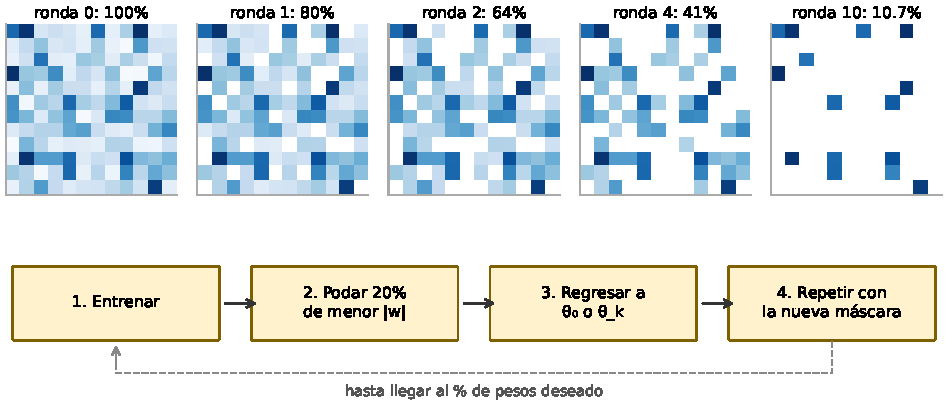
\includegraphics[width=0.85\textwidth]{imp.pdf}
\caption{Poda por magnitud iterativa (IMP). Arriba, los pesos de una capa ilustrativa (12$\times$12 valores aleatorios; más oscuro = mayor $|w|$, blanco = podado) tras 0, 1, 2, 4 y 10 rondas: con $p=20\%$ quedan $0.8^n$ de los pesos. Abajo, el ciclo. En el paso 3 el valor de referencia define la variante: $\theta_0$ (ticket), $\theta_k$ (rewinding) o pesos nuevos al azar (control). Es un esquema, no una corrida real.}
\label{fig:imp}
\end{figure}

\subsection{Resultados esperados}
\begin{itemize}[nosep]
    \item \textbf{Existencia (H0):} la curva del ticket se mantiene a menos de 1 punto de la red densa o por encima, y por encima de la curva aleatoria con un margen mayor al ruido.
    \item \textbf{Rewinding (H1):} si el ticket desde $\theta_0$ no supera al control pero el ticket con rewind sí, hace falta rewind.
    \item \textbf{Alcance de la poda (H3):} si la caída del ticket a poca densidad desaparece al cambiar de poda por capa a poda global con todo lo demás igual.
\end{itemize}

\subsection{Alcance de la poda}
En la poda \textit{por capa} cada capa pierde exactamente la misma fracción. Las capas pequeñas (como la primera convolución, con 1,728 pesos) quedan con muy pocos pesos en términos absolutos, mientras que las capas grandes (la primera capa lineal de la CNN tiene 2.1~M pesos, el 86\% del total) pierden en proporción lo mismo aunque sean redundantes. La poda \textit{global} compara las magnitudes de todos los pesos con un único umbral, de modo que cada capa conserva lo que su magnitud justifica. El riesgo opuesto es que una capa se quede sin pesos (\textit{layer collapse}); aquí se mide con filtros y neuronas completamente vacíos.

\subsection{Rewinding y warmup}
Frankle et~al.\ \cite{frankle2019stabilizing} muestran que en ResNet-18 y VGG-19 con \textit{learning rate} 0.1 el ticket desde $\theta_0$ no es mejor que la reinicialización, pero hacer rewind a una iteración temprana (cientos de iteraciones) sí lo es. Frankle y Carbin \cite{frankle2019lth} (apéndice) reportan que en esas redes aparecen tickets con un \textit{learning rate} menor o con warmup largo. Esto sugiere que el rewinding y el warmup atacan el mismo problema: el arranque del entrenamiento con un \textit{learning rate} alto es inestable y los pesos iniciales aún no están en una región donde la máscara sea estable. Esta es la base de H2; en este proyecto no se manipuló el warmup, solo se observó su coincidencia con la necesidad de rewinding en cada arquitectura (Sección~\ref{sec:h2}).

\subsection{Trabajo relacionado y límites de la comparación}
Para los ViT, Shen et~al.\ \cite{shen2023dlth} reportan que los tickets a nivel de peso son difíciles de encontrar en DeiT-Small con ImageNet; el ViT de este proyecto es pequeño y se entrena en CIFAR-10, así que sus resultados no son comparables directamente. Renda et~al.\ \cite{renda2020} comparan el rewinding con el ajuste fino tras la poda; aquí solo se toma su receta (SGD con \textit{weight decay} en ResNets de CIFAR-10) como referencia. El recipe de entrenamiento del ViT sigue las pautas de DeiT \cite{touvron2021deit} (AdamW, \textit{weight decay} 0.05, warmup), con las desviaciones del Apéndice~\ref{app:desv}.

\newpage
%% ======================================================================
\section{Propuesta de solución}
Para contestar las preguntas se diseñó una serie de experimentos que comparten el mismo código de poda (\texttt{lth.py}) y varían la arquitectura, el punto de rewind y el alcance de la poda. Cada experimento mide las tres curvas de la Sección~2.1 (ticket, ticket con rewinding, control aleatorio) contra el porcentaje de pesos restantes.

\begin{table}[H]
\centering\small
\begin{tabularx}{\textwidth}{@{}llYYYr@{}}
\toprule
Exp. & Arquitectura / datos & Poda & Rewind & Hipótesis que prueba & Épocas/ronda \\
\midrule
01 & MLP LeNet-300-100 / MNIST & capa & -- & H0 & 5 \\
02 & CNN Conv-4 / CIFAR-10 & capa & -- & H0, H3 & 30 \\
02b & CNN Conv-4 / CIFAR-10 & \textbf{global} & -- & \textbf{H3} & 30 \\
03 & ResNet de 20 capas / CIFAR-10 & global & época 1 & H0, H1, (H2) & 77 \\
04 & ViT pequeño / CIFAR-10 & global & época 2 & H0, H1, (H2) & 20 \\
05 & ViT, entrenamiento largo & global & época 5 & H0, H1, (H2) & 100 \\
\bottomrule
\end{tabularx}
\caption{Matriz de experimentos. (H2) indica que el warmup solo se observa, no se manipula.}
\end{table}

\paragraph{Enfoque del estudio.} El proyecto no estudia las cuatro arquitecturas con la misma profundidad. El \textbf{ViT} es la arquitectura a la que se dedicó más trabajo: dos corridas (20 y 100 épocas) con las tres curvas, validación de su baseline y la inspección completa de los checkpoints (pesos vivos por capa, accuracy por clase y atención). La \textbf{CNN} es el caso donde se comparó directamente la poda por capa y la global, con inspección de máscaras. El MLP y la ResNet sirven como puntos de referencia (una corrida cada uno, la ResNet con rewinding).

\paragraph{Cambios deliberados entre experimentos.} 02b cambia \textit{solo} el alcance de la poda respecto a 02. 05 repite 04 con 100 épocas, más aumento de datos y \textit{label smoothing} porque el baseline de 04 (78.9\%) parecía subentrenado y eso podría explicar que el ticket superara a la red densa. El ViT se mide dos veces (04 y 05) para separar el efecto de la poda del de un mal baseline.

\paragraph{Criterios de calidad.} Cada curva se compara con la accuracy de su red densa y con el control aleatorio; la inspección de las máscaras y de las redes sirve para explicar las diferencias, no para reemplazar la medición. Se declara explícitamente que una sola semilla y ~10,000 imágenes de prueba permiten distinguir diferencias de unos 5 puntos, pero no de 1 punto o menos.

\newpage
%% ======================================================================
\section{Descripción de la solución}
\subsection{Arquitecturas}
Cada red tiene su diagrama (Figuras~\ref{fig:archmlp} a~\ref{fig:archvit}); en todos, el verde marca las capas cuyos pesos entran a la poda.

\Needspace*{4.2in}
\paragraph{MLP (LeNet-300-100).} $784\to300\to100\to10$ con ReLU; 266k pesos podables, 235k de ellos en la primera capa.
\begin{figure}[H]
\centering
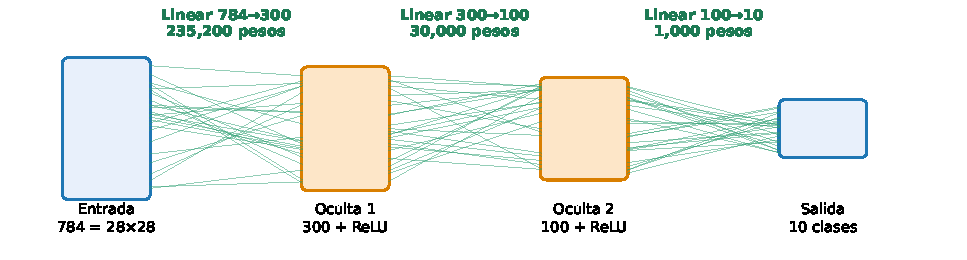
\includegraphics[width=0.92\textwidth]{arch_mlp.pdf}
\caption{MLP LeNet-300-100 para MNIST. Cada barra es una capa de neuronas y las líneas verdes son los pesos que se podan.}
\label{fig:archmlp}
\end{figure}

\Needspace*{3.3in}
\paragraph{CNN (Conv-4).} Cuatro convoluciones $3\times3$ (64, 64, 128, 128 filtros) con \textit{max-pooling} y tres capas lineales; 2.4M pesos, el 86\% en la primera capa lineal ($8192\to256$).
\begin{figure}[H]
\centering
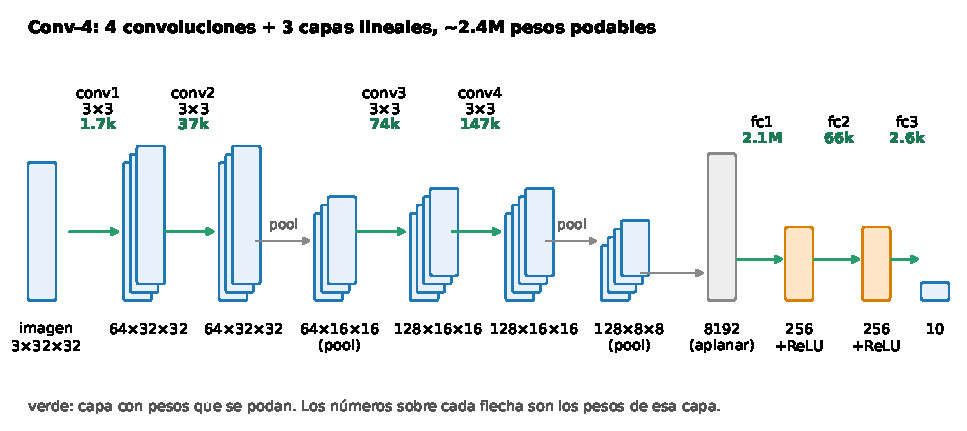
\includegraphics[width=0.92\textwidth]{arch_cnn.pdf}
\caption{CNN Conv-4 para CIFAR-10: forma de cada tensor y pesos de cada capa. La primera capa lineal concentra el 86\% de los pesos.}
\label{fig:archcnn}
\end{figure}

\Needspace*{3.6in}
\paragraph{ResNet de 20 capas.} Arquitectura del apéndice I.3 de \cite{frankle2019lth}: una convolución inicial y 9 bloques residuales en tres etapas de 16, 32 y 64 canales, con atajos convolucionales $1\times1$ cuando cambian las dimensiones; 270k pesos convolucionales. La capa lineal final no se poda.
\begin{figure}[H]
\centering
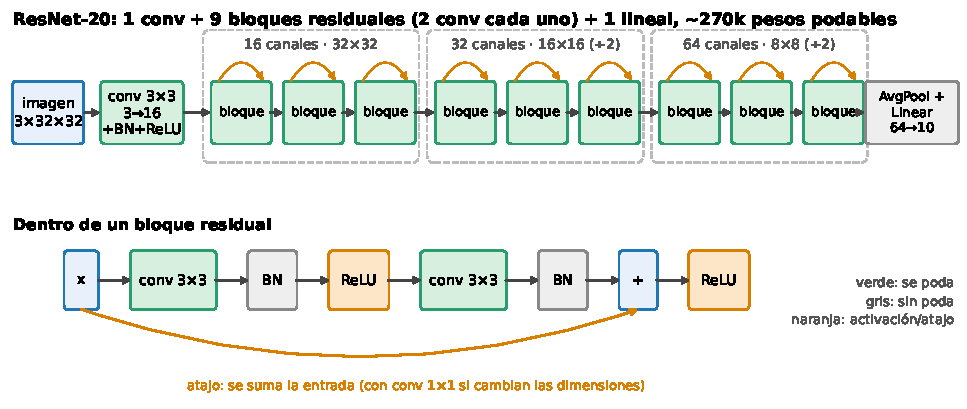
\includegraphics[width=0.92\textwidth]{arch_resnet.pdf}
\caption{ResNet de 20 capas. Arriba, la red completa (los arcos son los atajos residuales); abajo, el interior de un bloque.}
\label{fig:archresnet}
\end{figure}

\Needspace*{4.0in}
\paragraph{ViT pequeño.} Parches de $4\times4$ (64 tokens más \texttt{[CLS]}), dimensión 192, 6 bloques de atención con 3 cabezas y MLP de 384; 1.8M pesos podables. Todas las capas lineales y las LayerNorm entran en la poda global.
\begin{figure}[H]
\centering
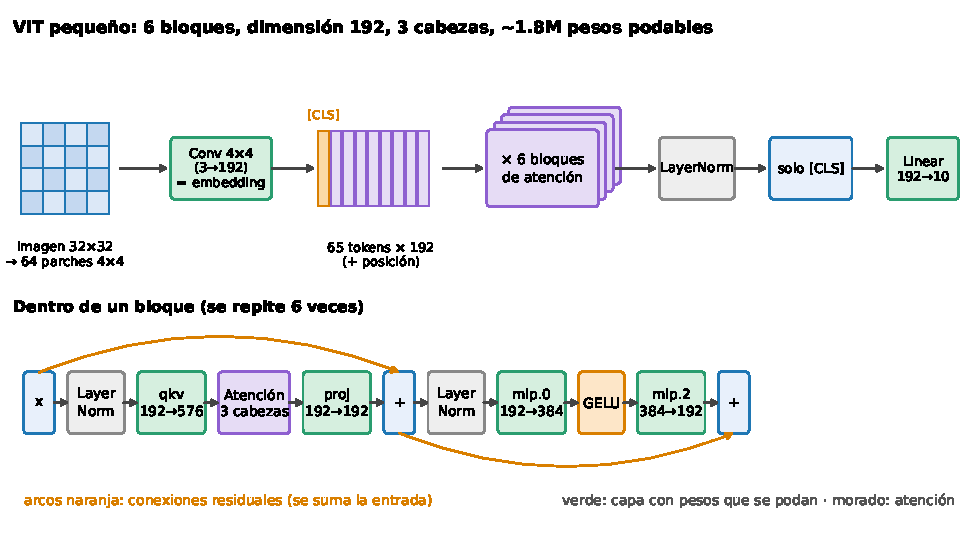
\includegraphics[width=0.92\textwidth]{arch_vit.pdf}
\caption{ViT pequeño. Arriba, de la imagen a la clasificación del token \texttt{[CLS]}; abajo, el interior de uno de los 6 bloques.}
\label{fig:archvit}
\end{figure}

El ciclo de poda (IMP) que se aplica a todas estas redes está en la Figura~\ref{fig:imp}.

\subsection{Implementación}
Los cuatro modelos, los ciclos de entrenamiento y evaluación y el módulo de poda \texttt{lth.py} fueron escritos por mí en PyTorch; el guardado de checkpoints y la mayor parte de los cuadernos de experimentos los implementó la IA (Sección~5.2). El módulo \texttt{lth.py} contiene:
\begin{itemize}[nosep]
    \item \texttt{run\_imp}: bucle de IMP con alcance \texttt{"layer"} o \texttt{"global"}, ritmo de poda configurable, rewind a la época $k$ y guardado de cada ronda;
    \item \texttt{run\_lth}: ejecuta las tres curvas (ticket, ticket con rewinding, control aleatorio con la misma máscara y otra inicialización);
    \item \texttt{save\_base}, \texttt{save\_round} / \texttt{list\_checkpoints} (implementados con IA): guardan pesos y máscaras de cada ronda para poder inspeccionarlos después sin reentrenar.
\end{itemize}
Los experimentos son notebooks \texttt{marimo} guardados como \texttt{.py} (reactivos y versionables), exportables a HTML. La comparación (06) y la inspección (07) leen los resultados guardados; la demo interactiva (08) usa los checkpoints para comparar modelos densos, tickets y controles sobre una imagen elegida.

\subsection{Hiperparámetros}
\begin{table}[H]
\centering\small
\begin{tabularx}{\textwidth}{@{}lYYYYY@{}}
\toprule
 & MLP & CNN & ResNet & ViT (04) & ViT largo (05) \\
\midrule
Optimizador & Adam 1.2e-3 & Adam 3e-4 & SGD 0.1, mom.\ 0.9 & AdamW 1e-3, wd 0.05 & igual \\
Aumento de datos & no & no & flip + crop & flip + crop & + RandAugment, erasing, mixup/cutmix, LS \\
Poda por ronda & 20\% capa & 20\% capa / global & 20\% global (solo conv.) & 35\% global & 35\% global \\
Rondas & 15 & 10 & 10 & 8 & 8 \\
Warmup & no & no & no & 2 ép.\ + coseno & 5 ép.\ + coseno \\
\bottomrule
\end{tabularx}
\caption{Configuración de cada experimento (LS = \textit{label smoothing}). Las desviaciones respecto a las fuentes están en el Apéndice~\ref{app:desv}.}
\end{table}

\subsection{Reproducibilidad y costo}
Entorno gestionado con \texttt{uv} (\texttt{uv.lock}); una sola semilla por experimento y entrenamiento en GPU (no determinista). Todo el proyecto usó unas 10 horas de GPU (RTX 4070 SUPER, ~4~kWh). Las figuras y tablas de este informe se generan con \texttt{report/make\_figures.py} a partir de \texttt{results/} y \texttt{checkpoints/}.

%% ======================================================================
\newpage
\section{Herramientas aplicadas}
\subsection{Herramientas}
\begin{itemize}[nosep]
    \item \textbf{PyTorch / torchvision}: modelos, entrenamiento y datasets (MNIST, CIFAR-10).
    \item \textbf{marimo}: cuadernos reactivos guardados como \texttt{.py}, exportables a HTML. Es una herramienta nueva para este curso (a diferencia de Jupyter, el orden de ejecución lo determina el grafo de dependencias entre celdas y el archivo es código normal, apto para git).
    \item \textbf{uv}: gestor de entornos reproducibles de Python.
    \item \textbf{Claude Code}: asistente de IA en la terminal, usado para leer el repositorio, ejecutar corridas, generar figuras de inspección y redactar borradores de análisis.
    \item \textbf{matplotlib}: figuras (el código de las figuras de inspección fue generado con ayuda de IA).
    \item \textbf{\LaTeX}: este informe; las figuras y tablas numéricas se generan por script.
\end{itemize}

\subsection{Uso de IA generativa: prompts y evolución de la idea}
\textit{Nota sobre los prompts: no se conserva un registro textual completo de la conversación con la IA. Lo que sigue son resúmenes de las interacciones más relevantes, redactados a partir de lo ocurrido en el proyecto; las frases entre comillas son citas textuales.}

\paragraph{Estrategia.} Primero se escribió a mano una ``implementación canónica'' (modelos, ciclos de entrenamiento y evaluación, y \texttt{lth.py}) para el MLP y la CNN. Con ella como referencia, se le pidió a la IA conectar \texttt{lth.py} al resto de los cuadernos, ejecutar los experimentos y agregar los experimentos extra. Funcionó porque la IA tenía un patrón concreto que copiar (misma estructura de cuaderno, mismas funciones de poda, mismas métricas) y porque cada resultado se podía comparar contra la implementación a mano. Los problemas aparecieron cuando se le pidió algo sin esa referencia o cuando agregó cosas no pedidas.

\textbf{Reparto.}

\textbf{Mío:} el tema, la pregunta y las hipótesis; los cuatro modelos (\texttt{nn.Module}); los ciclos de entrenamiento y evaluación; el código de poda \texttt{lth.py} (máscaras, IMP, control aleatorio); y ejecutar y verificar los experimentos. 

\textbf{De la IA (Claude, mediante Claude Code):} el guardado de pesos y máscaras (checkpoints); la implementación de la mayor parte de los cuadernos de experimentos, cuyas partes centrales el autor sabía correctas y revisó; las visualizaciones, los diagramas de arquitectura y las tablas automáticas; la revisión de código e hiperparámetros contra las fuentes; borradores de interpretación; y la estructura del informe y de la presentación.

\paragraph{Prompts de los que hay registro.}
\begin{itemize}[nosep]
    \item \textit{``Modify the notebooks to export the models so I can run experiments on them, using masks to see how they turn out.''} $\rightarrow$ origen del guardado de checkpoints (\texttt{save\_round}) y del cuaderno de inspección.
    \item \textit{``I wanna handpick from results to see what changes… also saving \% of original params and whatnot.''} $\rightarrow$ checkpoints por ronda con el porcentaje de pesos en el nombre.
    \item \textit{``ViT longer has to have more epochs + more aggressive data augmentation (Luego de una conversación más larga sobre el experimento como tal)''} $\rightarrow$ experimento 05.
\end{itemize}

\begin{table}[H]
\centering\footnotesize
\begin{tabularx}{\textwidth}{@{}>{\raggedright\arraybackslash}p{0.27\linewidth}>{\raggedright\arraybackslash}p{0.24\linewidth}Y@{}}
\toprule
Prompt (resumen) & Resultado & Evaluación y por qué \\
\midrule
Reescribir los cuadernos 01 y 02 con mejor markdown y documentación, manteniendo la estructura. & Una versión con opciones no pedidas (una variable de entorno para correr en modo rápido, celdas extra) y que ignoraba mi código. & \textbf{No satisfactorio.} La IA agregó complejidad y no siguió las convenciones de \texttt{marimo} (por ejemplo, \texttt{print(model)} en vez de dejar el modelo como última expresión de la celda). Se evaluó comparando contra mi código; se pidió rehacerlo partiendo de él, solo con markdown y partes comunes extraídas. \\
\midrule
Mover la lógica de poda a \texttt{lth.py}; los cuadernos solo cargan datos, definen el modelo, entrenan la versión inicial y llaman a \texttt{lth.py}. & Primero las máscaras se pasaban como parámetros y se usaban \textit{hooks} del optimizador; las funciones no se parecían a las mías. & \textbf{Falló al inicio, corregido después de insistir.} ``Los cuadernos quedan: cargar datos, modelo, entrenar versión inicial y guardar pesos; lo de poda y LTH va al archivo compartido''. Se validó revisando que las funciones fueran las mismas que ya tenía y que los cuadernos 01 y 02 quedaran con estructura equivalente. \\
\midrule
Agregar el guardado de checkpoints por ronda con el porcentaje de pesos en el nombre. & \texttt{save\_base}, \texttt{save\_round}, \texttt{list\_checkpoints} y el cuaderno de inspección. & \textbf{Satisfactorio.} Es una tarea acotada y fácil de verificar: se cargó un checkpoint y se comprobó que la máscara y el porcentaje coincidieran con lo reportado en las corridas. \\
\midrule
Correr el ViT con más épocas y más aumento de datos para validar el \textit{baseline} (experimento 05). & Cuaderno 05 con RandAugment, \textit{erasing}, mixup/cutmix y \textit{label smoothing}; la primera corrida del ViT denso se descartó y repitió. & \textbf{Satisfactorio con una corrección.} El cuaderno funcionó, pero la IA no había aplicado al 05 el arreglo de checkpoints que se le había pedido y hubo que repetir la instrucción. El resultado final se verificó contra el JSON de la corrida. \\
\midrule
Quitar los \texttt{print} del conteo de parámetros en los cuadernos. & La IA los volvió a agregar al tocar otro cuaderno. & \textbf{Error.} Revirtió una decisión deliberada. No se sabe por qué; se supone que la IA no tenía presente que esos \texttt{print} se habían quitado a propósito. Se detectó al ver el resultado y se pidió no volver a agregarlos. \\
\midrule
Correr la CNN con poda global (02b) para ver si el colapso se debe a la poda por capa. & Cuaderno 02b y los análisis de máscaras y de magnitud de pesos. & \textbf{Satisfactorio.} Antes de correrlo, el texto atribuía el colapso a la poda por capa como hecho; se reescribió como \textit{posible, no probada} hasta tener 02b. Después se verificó con las máscaras (0 filtros vacíos) y con los pesos por capa. \\
\midrule
Figuras de atención, gradientes y oclusión del ViT, y borradores de interpretación. & Mapas de atención y texto que decía que el control aleatorio ``mira abajo y por eso falla''. & \textbf{Parcialmente erróneo.} La atención no es una explicación (Jain y Wallace, 2019); se midió y su correlación con la oclusión fue $\approx 0$ (0.03 a 0.12). Se reescribió el texto, se marcó que las imágenes son elegidas a mano y se añadió la comparación atención contra oclusión. \\
\bottomrule
\end{tabularx}
\caption{Historial de prompts relevantes (resumido; las comillas son textuales).}
\end{table}

\paragraph{Evaluación crítica de la IA.} Todos los números que aparecen en el informe vienen de \texttt{results/*.json} o de los checkpoints; al crear la estructura del informe lo redactado con IA se marcó como \textit{borrador} y se contrastó con los datos antes de aceptarlo. Además, se tomó en cuenta que la IA puede dar explicaciones causales con una gran certeza a pesar de que los datos no lo apoyen. Por ejemplo, en algunos puntos había concluido una relación causal cuando el experimento simplemente fue observacional o utilizó los mapas de atención como explicación.

%% ======================================================================
\newpage
\section{Resultados}
\subsection{H0: existencia de tickets}
La Figura~\ref{fig:curves} muestra las curvas de todas las corridas y la Tabla~\ref{tab:summary} las resume. Las tres curvas son: ticket desde $\theta_0$ (azul), ticket con rewinding (verde) y reinicialización aleatoria de la misma máscara (naranja punteada).

\begin{figure}[H]
\centering
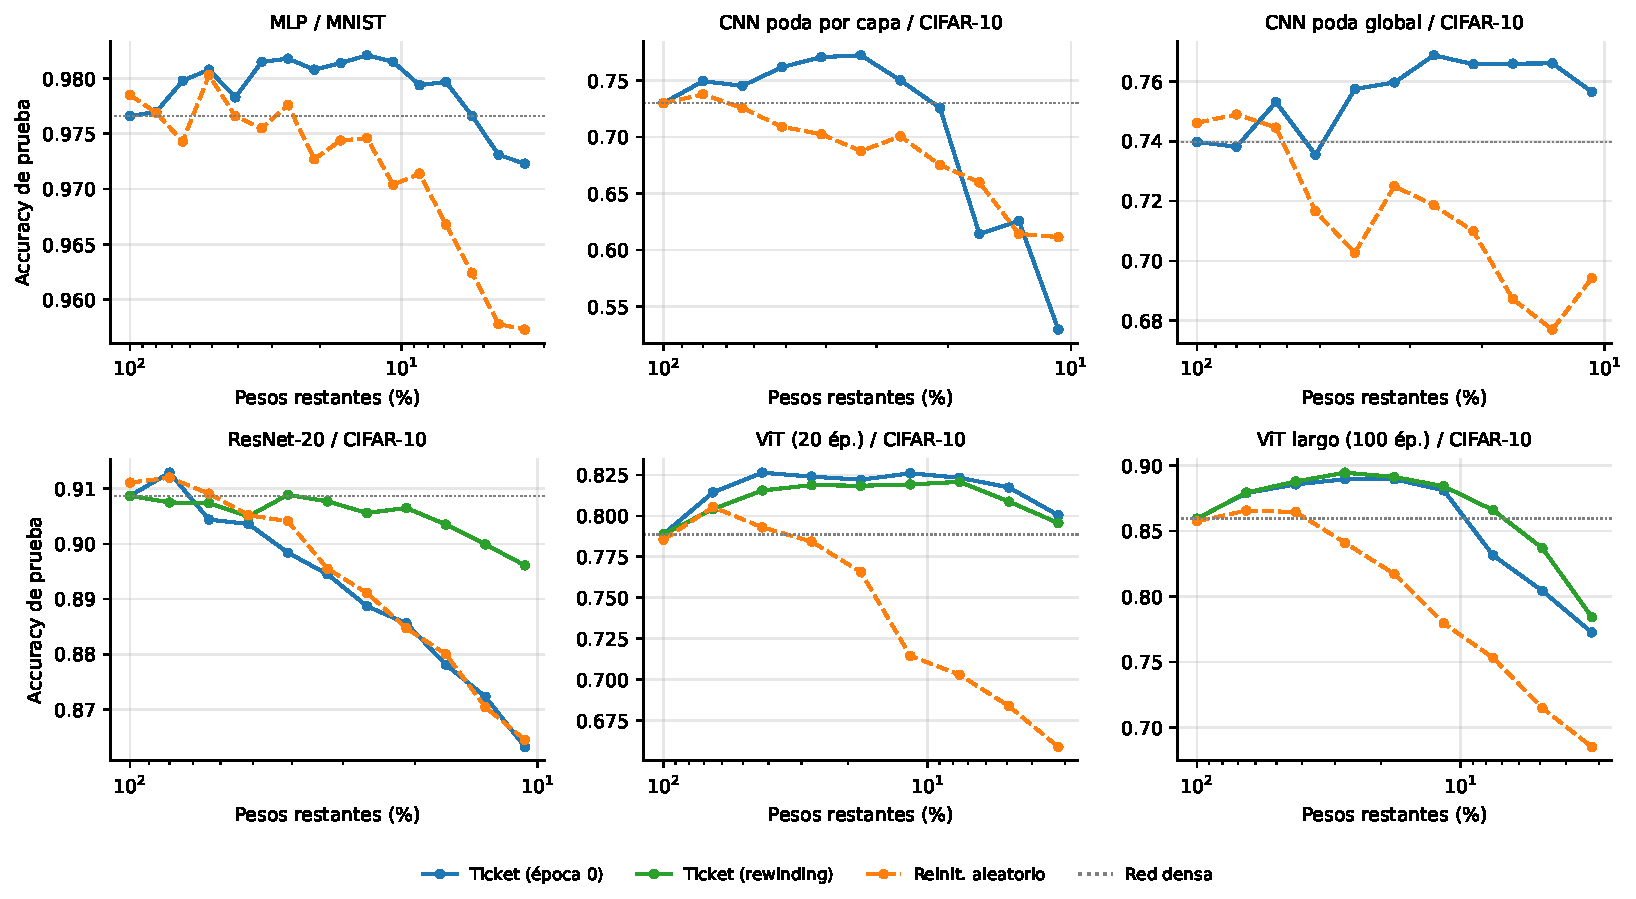
\includegraphics[width=\textwidth]{curves.pdf}
\caption{Accuracy de prueba contra porcentaje de pesos restantes (eje $x$ logarítmico e invertido: la red se hace más pequeña hacia la derecha).}
\label{fig:curves}
\end{figure}

\begin{table}[H]
\centering\footnotesize
\adjustbox{max width=\textwidth}{\begin{tabular}{@{}lrrrrr@{}}\toprule
Arquitectura & Densa (\%) & M\'in. pesos ticket & M\'in. pesos aleat. & Ventaja ticket (pts) & Ganancia rewind (pts) \\\midrule
MLP / MNIST & 97.7 & 3.5\% & 6.9\% & +0.8 & -- \\
CNN poda por capa / CIFAR-10 & 73.0 & 21.0\% & 64.0\% & +2.2 & -- \\
CNN poda global / CIFAR-10 & 74.0 & 10.7\% & 64.0\% & +4.4 & -- \\
ResNet-20 / CIFAR-10 & 90.9 & 51.2\% & 41.0\% & -0.1 & +1.5 \\
ViT (20 ép.) / CIFAR-10 & 78.9 & 3.2\% & 27.5\% & +8.1 & -0.7 \\
ViT largo (100 ép.) / CIFAR-10 & 86.0 & 11.6\% & 42.3\% & +6.4 & +1.1 \\
\bottomrule\end{tabular}
}
\caption{Resumen. ``Mín.\ pesos'': la red más pequeña a menos de 1 punto de la accuracy densa. ``Ventaja del ticket'': diferencia promedio entre el ticket y el control aleatorio sobre las rondas podadas. ``Ganancia del rewind'': diferencia promedio entre el ticket con rewinding y el clásico.}
\label{tab:summary}
\end{table}

\paragraph{MLP / MNIST.} El ticket se mantiene entre 97.2\% y 98.2\% hasta 3.5\% de los pesos, a la par de la red densa (97.7\%), mientras que la reinicialización aleatoria cae a 95.7\%. No se probó el rewinding. En la primera capa, 128 de los 784 píxeles de entrada quedan sin ningún peso (el borde de la imagen), lo cual es esperable porque los píxeles que siempre valen 0 no reciben gradiente.

\begin{figure}[H]
\centering
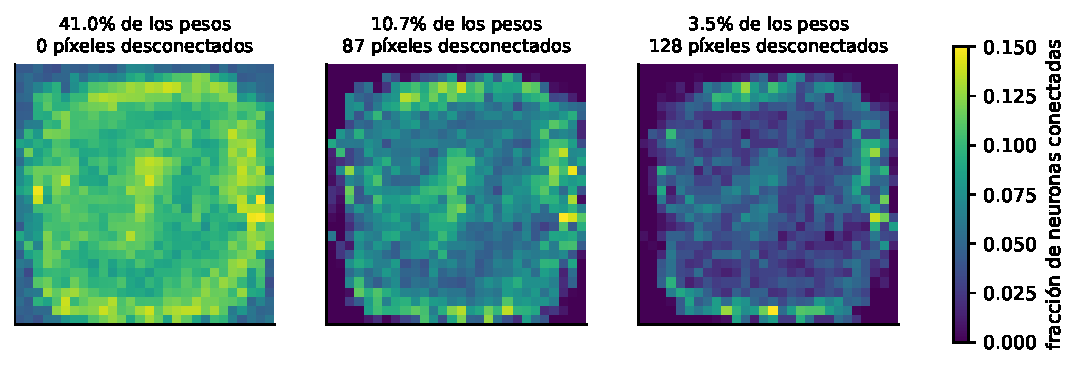
\includegraphics[width=0.85\textwidth]{mlp_mask.pdf}
\caption{MLP: para cada píxel de la imagen de $28\times28$, la fracción de las 300 neuronas ocultas que sigue conectada a él en la primera capa, en tres niveles de poda.}
\label{fig:mlpmask}
\end{figure}

Con 41\% de los pesos todavía todos los píxeles tienen alguna conexión; con 3.5\%, 128 píxeles del borde (donde los dígitos de MNIST casi siempre valen 0) quedan completamente desconectados y el resto se concentra en el centro de la imagen.

\paragraph{CNN / CIFAR-10.} Con poda por capa el ticket supera a la red densa (73.0\%) hasta con 26\% de los pesos, con un máximo de 77.2\% con 33--41\%, y supera al control hasta con 21\%; por debajo de eso cae a 61.4\% con 16.8\%, 62.6\% con 13.4\% y 53.0\% con 10.7\%, por debajo del control en 16.8\% y 10.7\% (ver Sección~\ref{sec:h3}). Con poda global el ticket se mantiene entre 73.6\% y 76.9\%, a la par o por encima de la red densa (74.0\%) en todo el rango y por encima del control desde 64\% de los pesos.

\paragraph{ResNet / CIFAR-10.} Con \textit{learning rate} 0.1 el ticket desde $\theta_0$ \textbf{no} supera al control (86.3\% frente a 86.5\% con 10.7\% de los pesos), igual que en \cite{frankle2019stabilizing}. Hacer rewind a la época 1 recupera casi toda la accuracy: 89.6\% con 10.7\% de los pesos (red densa: 90.9\%).

\paragraph{ViT / CIFAR-10.} Con 20 épocas el ticket queda en 82--83\% de 42\% a 7.5\% de los pesos, por encima de la red densa (78.9\%); el control cae a 65.9\% con 3.2\%. El baseline probablemente está subentrenado, motivo del experimento 05.

\subsection{ViT con entrenamiento largo}
El primer ViT (experimento 04, 20 épocas) quedó subentrenado: su red densa llegó a solo 78.9\%, y el ticket la superaba por varios puntos, lo que hacía sospechar que el resultado venía de un baseline débil y no de un ticket realmente bueno. Por eso se repitió con un entrenamiento largo (experimento 05: 100 épocas, warmup de 5 épocas y aumento de datos más fuerte). \textbf{Ese es el experimento principal del ViT}: es el que se usa para el resto del informe (rewinding, inspección de máscaras, atención), y el 04 queda como corrida preliminar.

\begin{figure}[H]
\centering
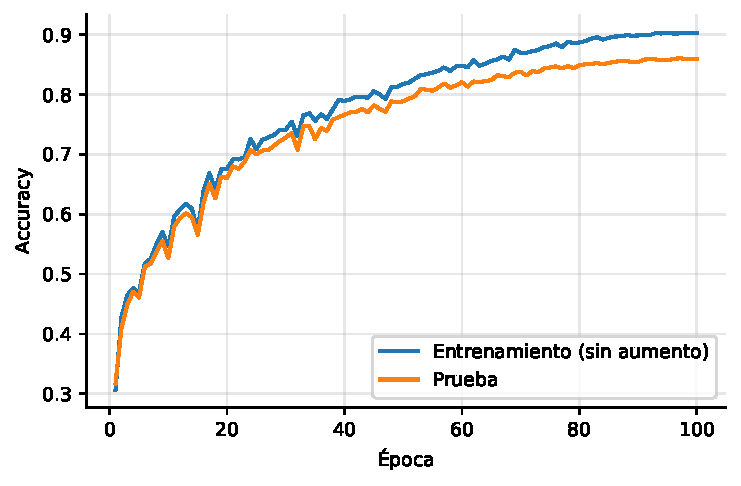
\includegraphics[width=0.55\textwidth]{vit_dense.pdf}
\caption{ViT denso de 100 épocas: accuracy de entrenamiento (sin aumento de datos) y de prueba por época.}
\label{fig:vitdense}
\end{figure}
Con 100 épocas la red densa llega a 86.0\% de accuracy de prueba (78.9\% en 04), con una brecha de unos 4 puntos respecto al entrenamiento y la prueba todavía subiendo: un baseline razonable. Medido otra vez desde otro arranque (ronda 0 del control aleatorio) da 85.7\%, así que la inicialización explica unos 0.2 puntos.

\begin{table}[H]
\centering\small
\adjustbox{max width=\textwidth}{\begin{tabular}{@{}rrrr@{}}\toprule
\% de pesos & Ticket $\theta_0$ & Ticket rewind (ép. 5) & Aleatorio \\\midrule
100.0 & 86.0 & 86.0 & 85.7 \\
65.0 & 87.9 & 87.9 & 86.6 \\
42.3 & 88.6 & 88.8 & 86.5 \\
27.5 & 88.9 & 89.5 & 84.1 \\
17.9 & 88.9 & 89.1 & 81.7 \\
11.6 & 88.1 & 88.4 & 78.0 \\
7.5 & 83.1 & 86.6 & 75.3 \\
4.9 & 80.4 & 83.7 & 71.5 \\
3.2 & 77.3 & 78.4 & 68.5 \\
\bottomrule\end{tabular}
}
\caption{ViT largo (05): accuracy de prueba (\%) por porcentaje de pesos restantes.}
\label{tab:vitlong}
\end{table}

El ticket sigue por encima de la red densa hasta $\sim$12\% de los pesos, así que el resultado de 04 no era solo un baseline débil. El ticket le gana al control aleatorio en todos los puntos, y la diferencia crece al podar más (de unos 5 puntos con 27.5\% de los pesos a unos 9 con 3.2\%).

\subsection{H1: rewinding según la arquitectura}
\begin{table}[H]
\centering\small
\begin{tabular}{@{}lll>{\raggedright\arraybackslash}p{0.38\linewidth}@{}}
\toprule
Arquitectura & Rewind probado & ¿Hizo falta? & Evidencia \\
\midrule
MLP & no & no & el ticket desde $\theta_0$ iguala a la red densa hasta 3.5\% de los pesos \\
CNN & no & no & ídem (con poda global hasta 10.7\%) \\
ResNet & época 1 & \textbf{sí} & desde $\theta_0$ igual al aleatorio (86.3 vs.\ 86.5\%); con rewind 89.6\% \\
ViT 20 ép. & época 2 & no & rewind queda $\approx$ ticket ($-0.7$ puntos en promedio) \\
ViT 100 ép. & época 5 & solo con poca densidad & sin efecto con $\ge$12\% de pesos; +3.4 puntos con 7.5\% y +3.3 con 4.9\%, +1.2 con 3.2\% \\
\bottomrule
\end{tabular}
\caption{Necesidad de rewinding por arquitectura.}
\end{table}

Los datos son compatibles con la idea de que a más complejidad se necesita hacer rewind (MLP y CNN no, ResNet sí), pero el ViT, la arquitectura más compleja, no lo necesita con densidades medias. La relación no es monótona en la complejidad; la explicación que más compite es H2 (Sección~\ref{sec:h2}).

En el ViT largo el rewinding solo ayuda cuando quedan pocos pesos, con 12\% o más la subred aún tiene capacidad para recuperarse desde cualquier inicialización razonable, y ticket, rewind y red densa quedan dentro de $\sim$1 punto. Con 7.5\% y 4.9\% la subred tiene poca capacidad y su entrenamiento es más sensible; Frankle et~al.\ \cite{frankle2019stabilizing} encuentran que el ticket solo es estable si se arranca después de unas pocas iteraciones. Las 5 épocas del rewinding coinciden con el final del warmup, lo que es compatible con esa idea pero no se probó. En 04 el baseline subentrenado dejaba poco margen, y no tiene los puntos 7.5\% y 4.9\% donde 05 muestra la ganancia; las dos corridas no son comparables punto por punto.

\subsection{H2: ¿hace falta warmup? (observacional)}\label{sec:h2}
La ResNet (sin warmup, \textit{learning rate} 0.1 desde la época 0) necesita rewinding; el ViT (con warmup de 2 y 5 épocas) funciona desde $\theta_0$ y solo aprovecha el rewind con muy poca densidad. Como el warmup no se varió dentro de una misma arquitectura, y las dos difieren además en optimizador, tipo de capas, etc., no se puede concluir que el warmup haga el trabajo del rewinding. Sin embargo, lo observado sí es compatible con esa hipótesis. Como prueba directa a futuro, se repetiría la ResNet con warmup y el ViT sin warmup: se esperaría que el ticket desde $\theta_0$ aparezca en la ResNet y desaparezca en el ViT.

\subsection{H3: poda por capa frente a poda global (CNN)}\label{sec:h3}
Con poda por capa el ticket de la CNN cae a partir de 16.8\% de los pesos y llega al mínimo con 10.7\%: 49.7\% frente a 61.0\% del control en la primera corrida, y 53.0\% frente a 61.2\% en la repetición (resultados de este informe), por lo que no es ruido. Con poda global (02b) el colapso desaparece: 75.7\% para el ticket frente a 69.4\% del control (red densa: 74.0\%). Pasa de 8 puntos \textit{por debajo} del control a 6 puntos \textit{por encima}.

\begin{figure}[H]
\centering
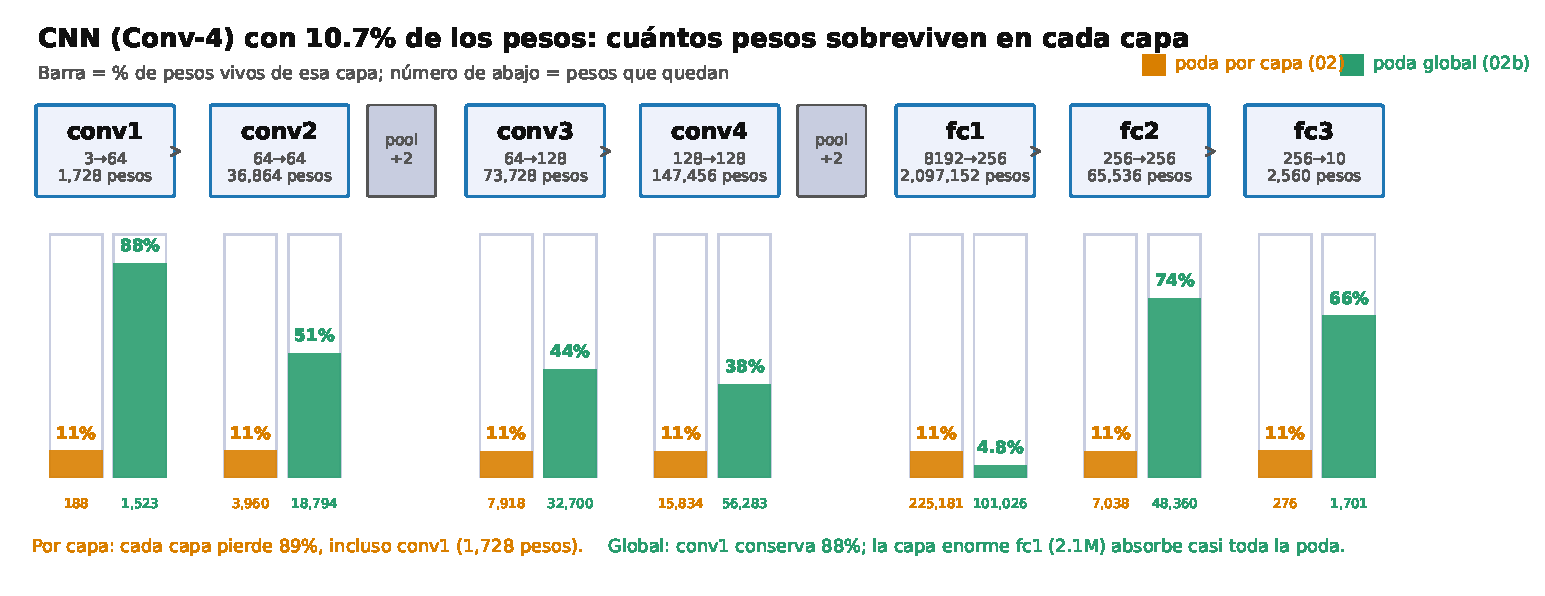
\includegraphics[width=\textwidth]{cnn_diagram.pdf}
\caption{La CNN (Conv-4) con 10.7\% de los pesos totales. Sobre cada capa: forma y número de pesos; debajo: fracción de pesos vivos de esa capa con poda por capa (naranja) y poda global (verde), y número de pesos que quedan. Con poda por capa todas las capas quedan en $\sim$11\%; con poda global conv1 conserva 88\% y fc1 solo 4.8\%.}
\label{fig:cnndiagram}
\end{figure}

\begin{figure}[H]
\centering
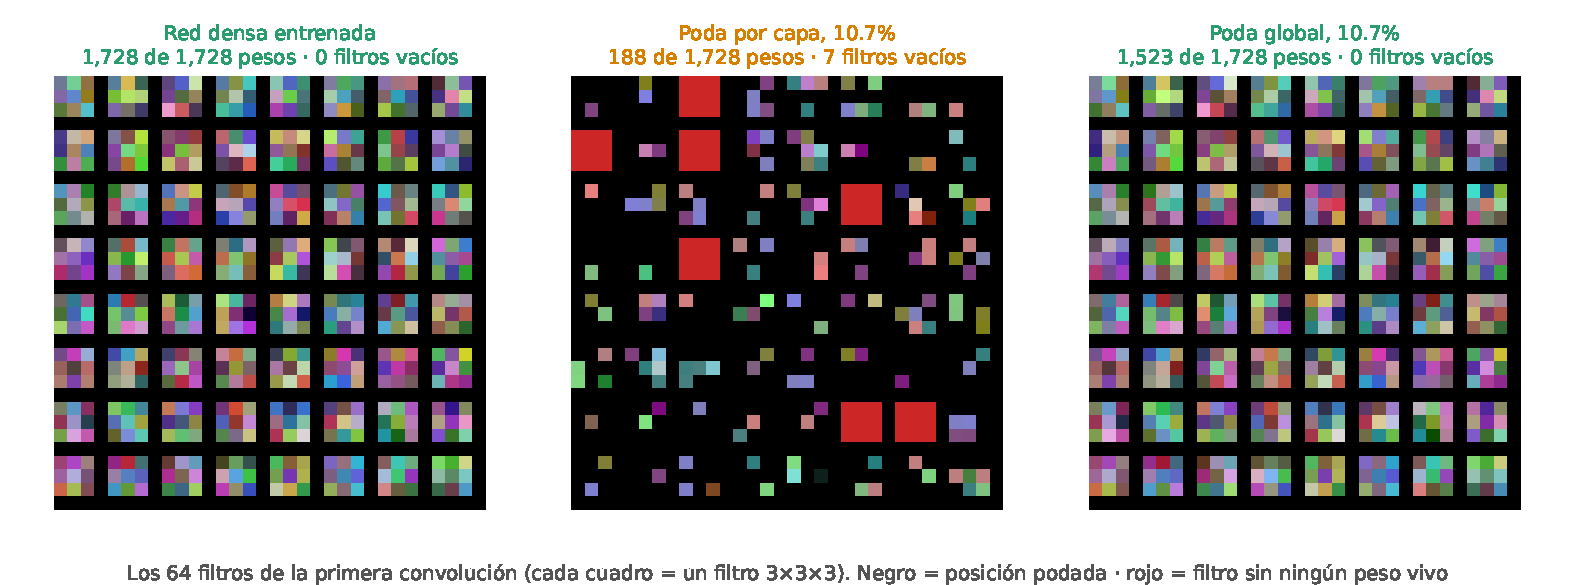
\includegraphics[width=\textwidth]{cnn_filters.pdf}
\caption{Los 64 filtros de la primera convolución de la red densa, del ticket con poda por capa y del ticket con poda global (10.7\% de los pesos). Cada cuadro es un filtro $3\times3\times3$ (el color son los tres canales). Negro: posición podada. Rojo: filtro sin ningún peso vivo.}
\label{fig:cnnfilters}
\end{figure}

\begin{table}[H]
\centering\footnotesize
\adjustbox{max width=\textwidth}{\begin{tabular}{@{}lrrrrrr@{}}\toprule
 & \multicolumn{3}{c}{Por capa (02)} & \multicolumn{3}{c}{Global (02b)} \\\cmidrule(lr){2-4}\cmidrule(lr){5-7}
Capa & \% vivo & Pesos & Vac\'ios & \% vivo & Pesos & Vac\'ios \\\midrule
conv1 (3$\to$64) & 10.9 & 188 & 7/64 & 88.1 & 1\,523 & 0/64 \\
conv2 (64$\to$64) & 10.7 & 3\,960 & 0/64 & 51.0 & 18\,794 & 0/64 \\
conv3 (64$\to$128) & 10.7 & 7\,918 & 0/128 & 44.4 & 32\,700 & 0/128 \\
conv4 (128$\to$128) & 10.7 & 15\,834 & 0/128 & 38.2 & 56\,283 & 0/128 \\
fc1 (8192$\to$256) & 10.7 & 225\,181 & -- & 4.8 & 101\,026 & -- \\
fc2 (256$\to$256) & 10.7 & 7\,038 & -- & 73.8 & 48\,360 & -- \\
fc3 (256$\to$10) & 10.8 & 276 & 102/256 & 66.4 & 1\,701 & 0/256 \\
\bottomrule\end{tabular}
}
\caption{CNN, ronda 10 (10.7\% de los pesos). ``Vacíos'': filtros convolucionales sin ningún peso vivo; en fc3, neuronas ocultas sin ningún peso hacia la salida.}
\label{tab:cnnmasks}
\end{table}

Con poda global la primera convolución conserva 88\% de sus pesos, no hay filtros ni neuronas vacíos (Tabla~\ref{tab:cnnmasks}) y la primera capa lineal, que tiene 86\% de los pesos, queda en 4.8\%. Con poda por capa hay 7 filtros vacíos en conv1 y 102 de las 256 neuronas ocultas no llegan a la salida.

\paragraph{Limitaciones.} Una sola corrida por configuración, con inicializaciones distintas en 02 y 02b y dense baselines de 73.0\% y 74.0\% (el ruido entre corridas es de $\sim$1 punto). Además, 02b cambia a la vez el alcance de la poda y cuántos pesos conserva cada capa; no separa ambas cosas.

\subsection{Inspección del ViT largo}
Checkpoints de 05 a 11.6\% de los pesos (ronda 5). \texttt{07\_inspection} tiene vistas adicionales (cabezas de atención, IoU entre ticket y rewinding, forma de las máscaras).

\paragraph{Pesos vivos por capa.}
\begin{figure}[H]
\centering
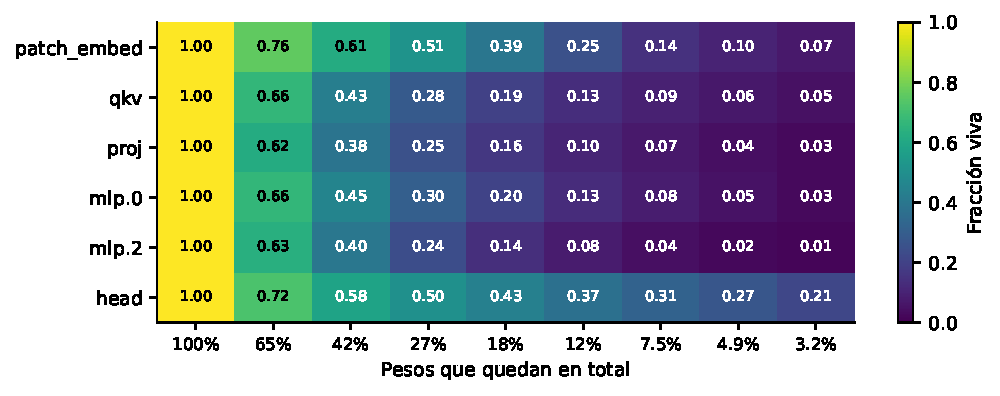
\includegraphics[width=0.85\textwidth]{heat.pdf}
\caption{ViT largo: fracción viva por tipo de capa y ronda de poda (promedio ponderado sobre los 6 bloques).}
\label{fig:heat}
\end{figure}
Clara = casi todos los pesos vivos. En la última ronda (3.2\% del total) \texttt{head} conserva 21\%, \texttt{patch\_embed} 7\%, \texttt{qkv} 4.5\%, \texttt{mlp.0} 2.7\%, \texttt{proj} 2.6\% y \texttt{mlp.2} 1.3\%.

\begin{figure}[H]
\centering
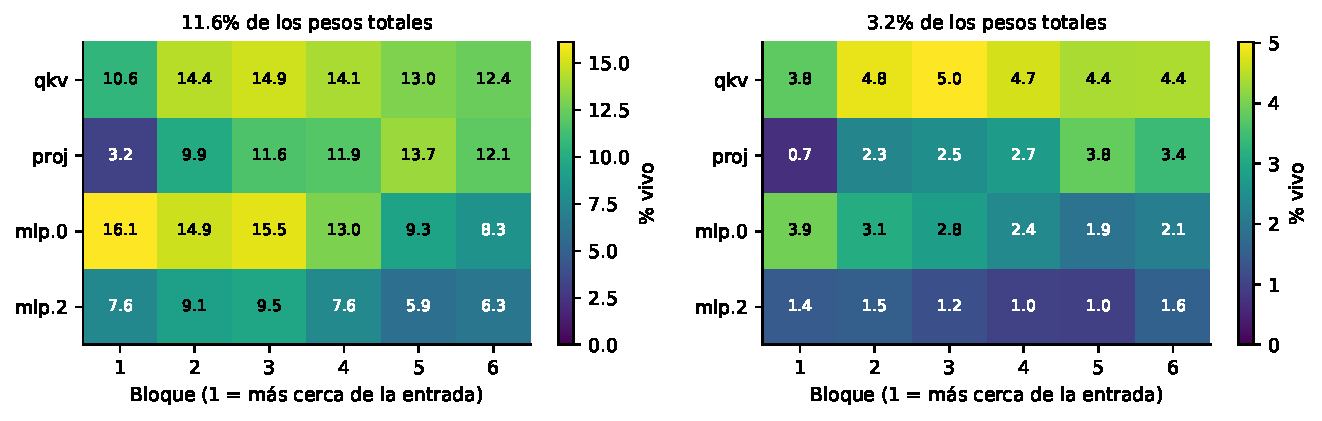
\includegraphics[width=\textwidth]{vit_depth.pdf}
\caption{ViT largo: porcentaje de pesos vivos de cada capa dentro de cada bloque (1 = el más cercano a la entrada), con 11.6\% y 3.2\% de los pesos totales.}
\label{fig:vitdepth}
\end{figure}
Cada celda es una capa de un bloque. \texttt{mlp.0} conserva menos pesos en los bloques tardíos (16.1\% en el bloque 1 y 8.3\% en el 6 con 11.6\%), \texttt{proj} lo contrario (3.2\% a 12.1\%) y \texttt{qkv} es casi plano. \texttt{proj} del bloque 1 queda en 0.7\% con 3.2\% de los pesos.

\begin{figure}[H]
\centering
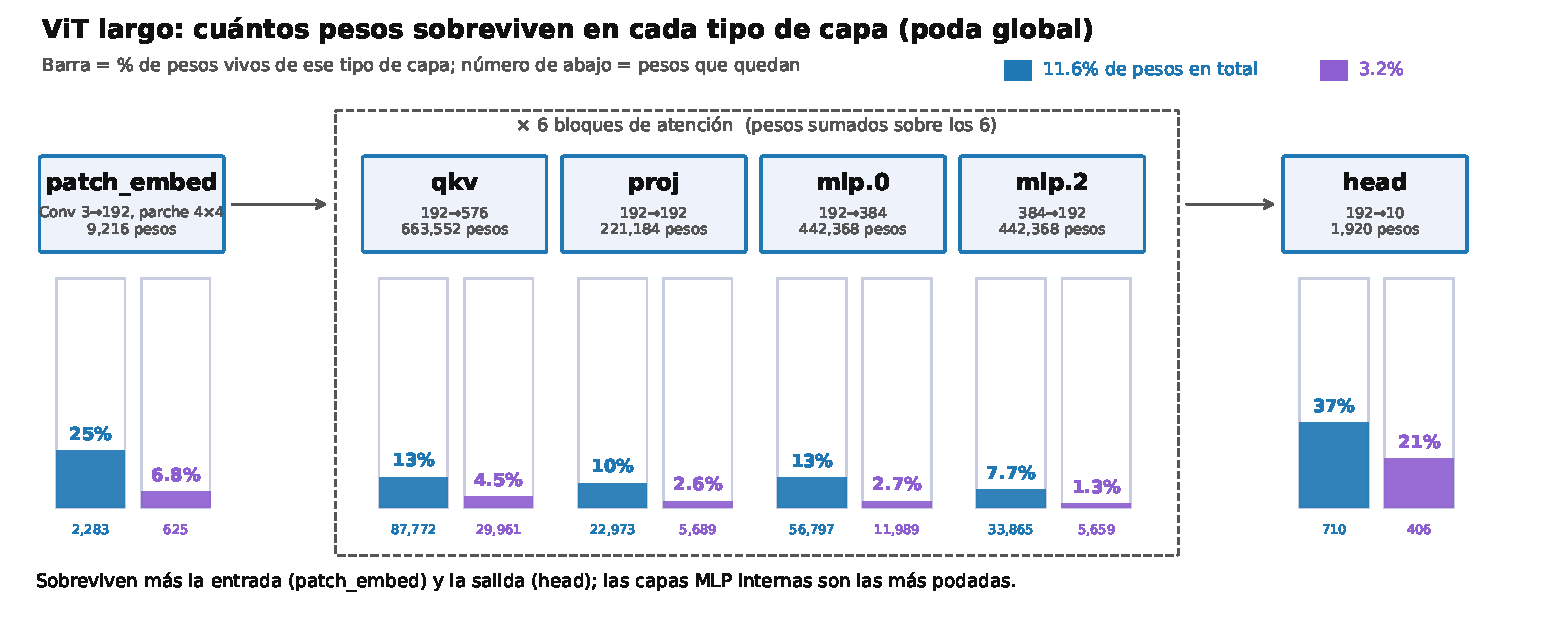
\includegraphics[width=\textwidth]{vit_diagram.pdf}
\caption{ViT largo: fracción de pesos vivos por tipo de capa (sumados sobre los 6 bloques) con 11.6\% y con 3.2\% de los pesos totales, y número de pesos que quedan.}
\label{fig:vitdiagram}
\end{figure}
Misma información que el mapa de calor, ordenada como la red. Las capas extremas conservan más y \texttt{mlp.2} es la más podada.

\paragraph{Accuracy por clase.}
\begin{figure}[H]
\centering
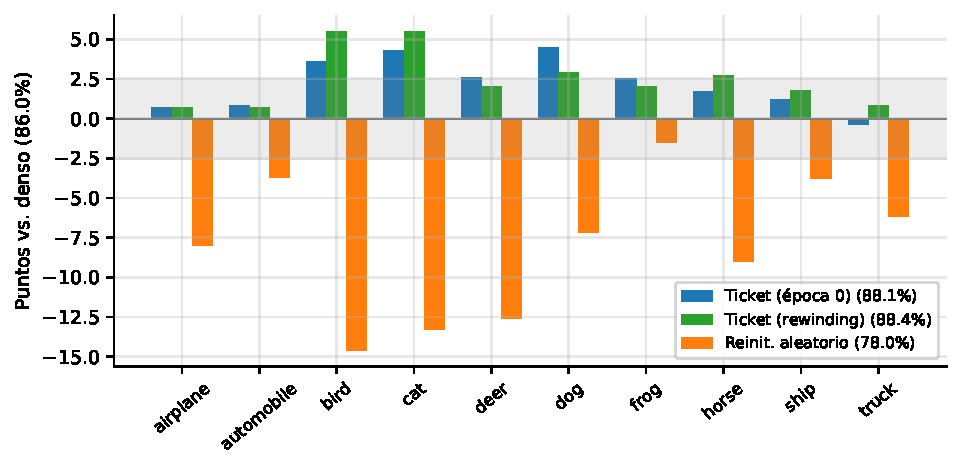
\includegraphics[width=0.75\textwidth]{cls.pdf}
\caption{ViT largo: diferencia de accuracy por clase respecto al denso (11.6\% de los pesos). Banda gris: ruido de $\pm2.5$ puntos.}
\label{fig:cls}
\end{figure}
Positivo = acierta más que el denso en esa clase; solo cuenta lo que sale de la banda gris (1,000 imágenes por clase). El ticket queda entre $-0.4$ y $+4.5$ puntos del denso, el rewinding entre $+0.7$ y $+5.5$ y el control pierde en todas las clases (hasta 14.6 puntos en pájaro).

\paragraph{Atención y oclusión.} Los mapas de atención del \texttt{[CLS]} (último bloque, promedio de cabezas) se suelen leer como ``dónde mira el modelo'', y la idea era usarlos para ver qué conserva el ticket y qué pierde el control aleatorio. Pero la atención no siempre refleja qué usa el modelo para decidir (Jain y Wallace, 2019), así que antes de interpretarla se comparó con una medida más directa, la oclusión: se tapa cada parche con el color medio de la imagen y se mide cuánto baja la probabilidad de la clase correcta. Se hizo con 150 imágenes de prueba y los cuatro modelos a 11.6\% de los pesos.

\begin{figure}[H]
\centering
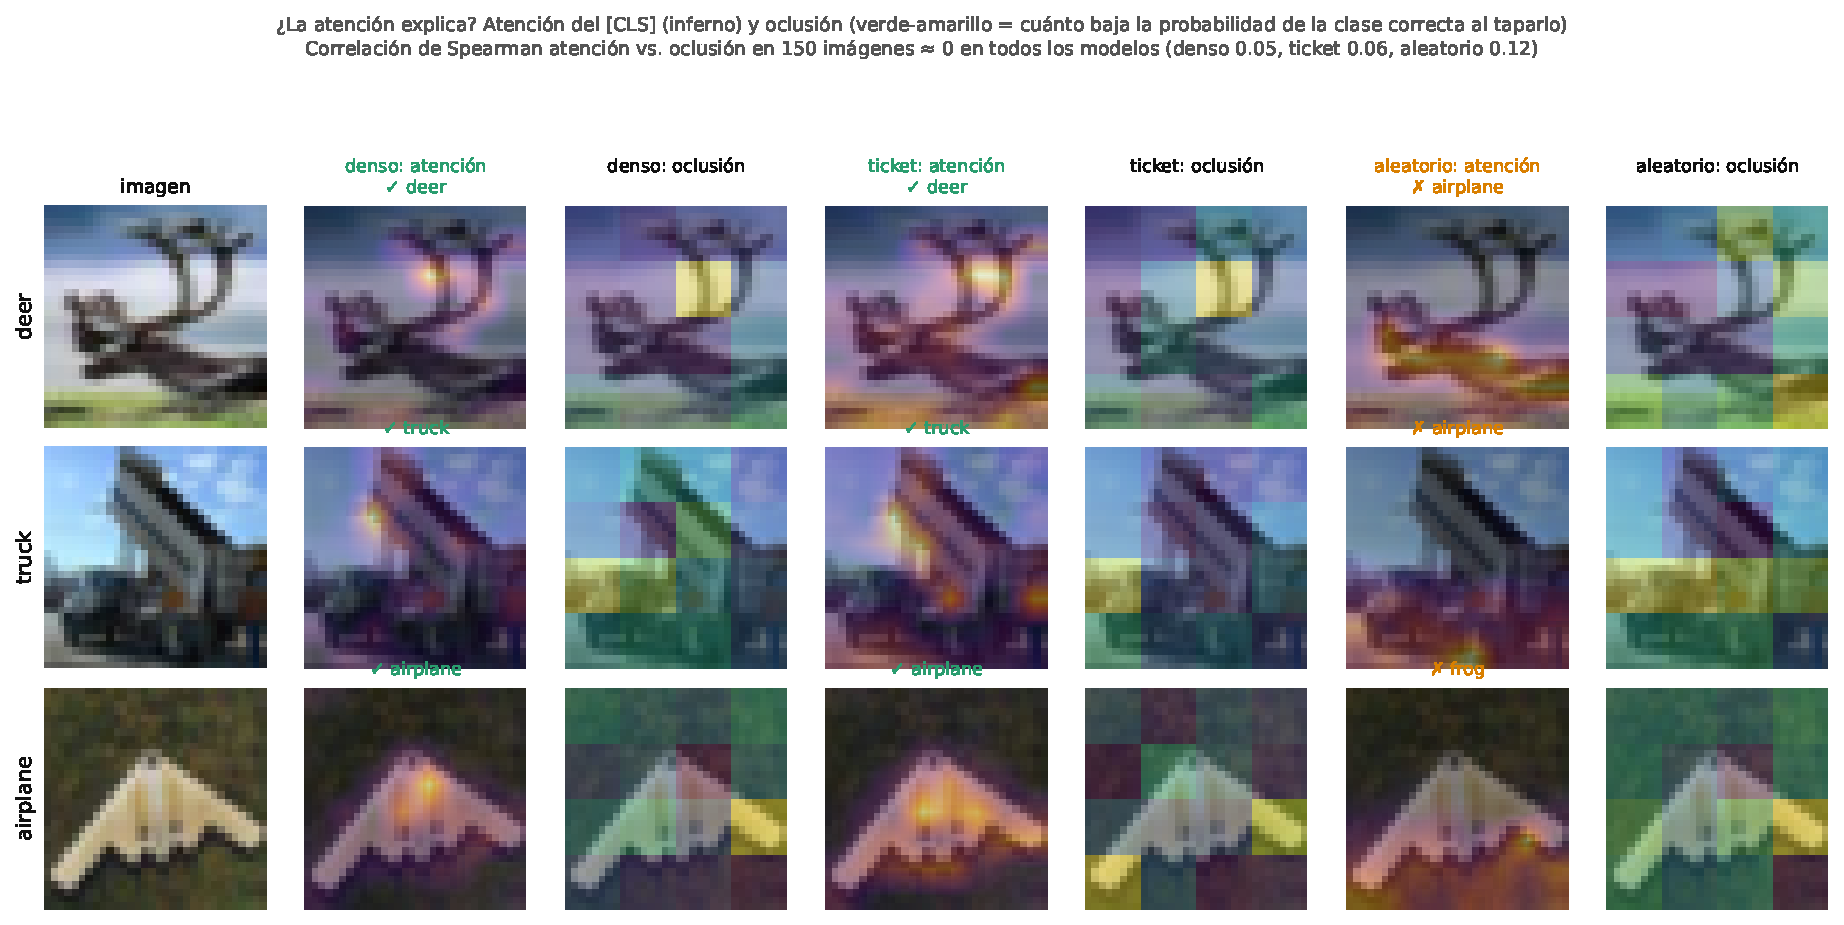
\includegraphics[width=\textwidth]{vit_occlusion.pdf}
\caption{Atención del \texttt{[CLS]} y oclusión de bloques de $8\times8$ píxeles (amarillo = al taparlo baja más la probabilidad de la clase correcta) para el denso, el ticket y el control aleatorio, con 11.6\% de los pesos. \textbf{Las tres imágenes están elegidas}: son de las 140 (entre las primeras 1{,}500 de prueba) en las que denso, ticket y rewinding aciertan y el control falla; no son representativas.}
\label{fig:vitocc}
\end{figure}

\textbf{Hallazgo 1: la atención no coincide con la oclusión.} La correlación de Spearman entre ambas es $\approx0$ en los cuatro modelos: 0.05 (denso), 0.06 (ticket), 0.03 (rewinding) y 0.12 (aleatorio) con bloques de $8\times8$; con $4\times4$, 0.01, 0.03, 0.01 y 0.07; con \textit{attention rollout}, 0.04 a 0.09. Los parches a los que más atiende el modelo no son los que más afectan la predicción al taparlos, así que los mapas de atención se presentan como descripción y no se usan para explicar nada.

\textbf{Hallazgo 2: los mapas del control aleatorio son distintos.} Los mapas del denso, el ticket y el rewinding se parecen entre sí (Tabla~\ref{tab:mapsim}: 0.63 a 0.73 en atención y 0.48 a 0.55 en oclusión); los del control casi no se parecen a los demás en atención (0.17 a 0.28) y se parecen menos en oclusión (0.33 a 0.35). Es un resultado raro: el control comparte la máscara con el ticket y aun así cambia bastante, y como la atención no explica la decisión no se puede decir por qué. Solo se registra que es distinto. Una reserva: denso, ticket y rewinding comparten $\theta_0$ y el control no, y no hay referencia de cuánto se parecen dos redes densas entrenadas por separado (cifras en \texttt{results/map\_similarity.json}).

\begin{table}[H]
\centering\small
\begin{tabular}{@{}lrr@{}}\toprule
Par de modelos & Atenci\'on & Oclusi\'on \\\midrule
denso -- ticket & 0.63 & 0.48 \\
denso -- rewinding & 0.70 & 0.49 \\
ticket -- rewinding & 0.73 & 0.55 \\
\midrule
denso -- control aleatorio & 0.17 & 0.35 \\
ticket -- control aleatorio & 0.28 & 0.35 \\
rewinding -- control aleatorio & 0.24 & 0.33 \\
\bottomrule\end{tabular}

\caption{Correlación de Spearman media entre los mapas de dos modelos (11.6\% de los pesos, 150 imágenes de prueba; 1 = mismo orden). Una sola corrida por modelo; la oclusión con color medio puede introducir artefactos.}
\label{tab:mapsim}
\end{table}

\newpage
%% ======================================================================
\section{Discusión}
\subsection{Discusión por hipótesis}
\paragraph{H0, existencia de tickets: apoyada.} En las cuatro arquitecturas hay una subred pequeña que iguala o supera a la red densa y le gana al control aleatorio: en el MLP hasta 3.5\% de los pesos (97.7\% la red densa), en la CNN con poda global hasta 10.7\% (75.7\% frente a 74.0\%) y en el ViT largo hasta $\sim$12\% (por encima del denso de 86.0\%). En la ResNet solo aparece con rewinding: 89.6\% con 10.7\% de los pesos, frente a 90.9\% del denso y 86.3\% desde $\theta_0$. Que el ticket supere al denso en el ViT puede ser un efecto regularizador de la poda; no se probó. Todo con una semilla (ver Limitaciones).

\paragraph{H1, complejidad y rewinding: parcial.} La ResNet necesita rewinding; el MLP, la CNN y el ViT de 20 épocas no; el ViT largo solo con poca densidad (+3.4 puntos con 7.5\% de los pesos y +3.3 con 4.9\%). La relación no es monótona con la complejidad, porque el ViT, la más compleja, no lo necesita con densidades medias. Cada arquitectura tiene uno o dos puntos de rewind y difieren en más que su complejidad (datos, optimizadores y \textit{schedules}, alcance y tasa de poda, épocas), así que los datos son compatibles con la hipótesis de forma cualitativa pero no la prueban.

\paragraph{H2, warmup y rewinding: compatible, no probada.} La ResNet (sin warmup, \textit{learning rate} 0.1) necesita rewinding y el ViT (con warmup) funciona desde $\theta_0$, lo que concuerda con que el warmup haga el trabajo del rewinding. Pero el warmup nunca se varió dentro de una misma arquitectura, y las dos difieren en optimizador, normalización y datos. La prueba directa sería la ResNet con warmup y el ViT sin él.

\paragraph{H3a, poda global frente a por capa (CNN): apoyada.} Con poda por capa el ticket colapsa con 10.7\% de los pesos (53.0\% frente a 61.2\% del control); con poda global no (75.7\% frente a 69.4\%). Las máscaras muestran el mecanismo: con poda global conv1 conserva 88\% de sus pesos y no hay filtros ni neuronas vacíos; con poda por capa hay 7 filtros vacíos. El resultado también afecta la comparación entre arquitecturas: el MLP y la primera CNN podaron por capa y la ResNet y el ViT globalmente, así que parte de lo que parece una diferencia entre arquitecturas puede ser una diferencia entre tipos de poda. La limitación principal es que 02b cambia a la vez el alcance de la poda y cuántos pesos conserva cada capa; el experimento no separa ambas cosas.

\paragraph{Tamaño de los pesos.}\label{sec:magnitudes} La poda global quita los pesos más pequeños de toda la red, así que lo que sobrevive en cada capa depende de qué tan grandes son sus pesos. En la CNN, los pesos de conv1 son unas 12 veces más grandes que los de fc1 (mediana de 0.105 frente a 0.0086): conv1 tiene solo 1,728 pesos y fc1 más de 2 millones. Un umbral global tira primero los de fc1 y casi no toca conv1; la poda por capa obliga a conv1 a perder lo mismo que fc1, y eso deja filtros y neuronas vacíos. En el ViT pasa algo parecido pero menos claro: \texttt{head} y \texttt{patch\_embed} tienen los pesos más grandes y sobreviven más.

\begin{figure}[H]
\centering
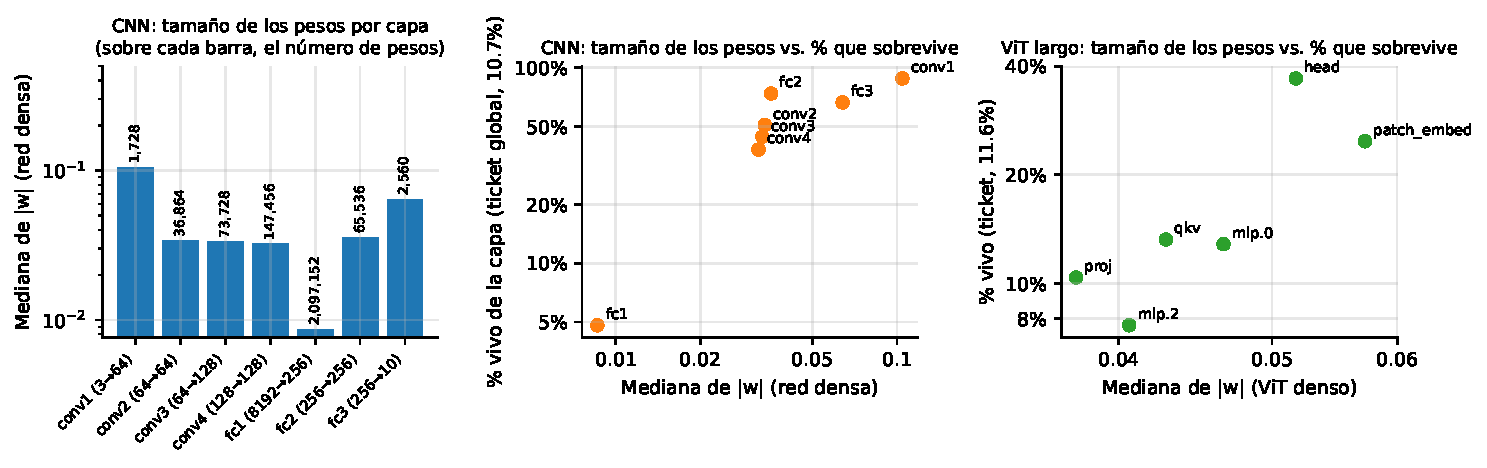
\includegraphics[width=\textwidth]{magnitudes.pdf}
\caption{Tamaño de los pesos de cada capa en la red densa y fracción que sobrevive a la poda global. Izquierda: cada barra es una capa de la CNN (sobre la barra, su número de pesos). Centro y derecha: cada punto es una capa de la CNN (10.7\% de los pesos) o un tipo de capa del ViT (11.6\%); más a la derecha = pesos más grandes, más arriba = más pesos vivos. Una sola corrida: es una asociación, no una prueba.}
\label{fig:mag}
\end{figure}

\paragraph{H3b, redes grandes necesitan poda global: consistente, no probada.} Con la CNN se puede concluir que la poda por capa causó el colapso y que el mecanismo es el cuello de botella en las capas pequeñas: tienen los pesos más grandes y se les obligó a perder la misma fracción que a la capa enorme y redundante. Eso \textit{no} prueba que toda red grande necesite poda global: ResNet y ViT no se podaron por capa; el MLP sí, sin problemas (97.2\% con 3.5\% de los pesos, aunque su capa de salida tiene 1,000 pesos); y la CNN, con una capa que concentra el 86\% de los pesos, es el caso más favorable para la poda global. Es razonable esperar que el problema crezca con la heterogeneidad de tamaños (el ViT va de 1,920 pesos en \texttt{head} a 442,368 en \texttt{mlp}, y \cite{frankle2019lth} usa poda global en las redes profundas), pero la prueba directa sería repetir el ViT (unos 45 min de GPU) y la ResNet (1 h 45 min) con poda por capa.

\paragraph{Inspección del ViT.} La poda global no es pareja: \texttt{head} y \texttt{patch\_embed} conservan más pesos y \texttt{mlp.2} es la más podada; dentro de los bloques, \texttt{mlp.0} pierde más en los tardíos y \texttt{proj} al revés. No se probó por qué. Por clase, el ticket queda dentro del ruido y el control aleatorio pierde en todas. Como la atención no predice la oclusión, lo que se puede decir del ViT sobre mapas de atención es descriptivo (Sección~6.6): los del control son distintos, pero no se sabe por qué.

\paragraph{Otras vistas revisadas.} Durante la inspección se generaron y se revisaron bastantes más gráficas de las que aparecen en este informe: atención por cabeza, entropía de la atención, gradientes en el paso 0, IoU entre las máscaras del ticket y del rewinding, forma de las máscaras y fracción viva por posición del kernel, si los pesos que sobreviven ya eran grandes en la inicialización, matrices de confusión y una imagen por clase. No se incluyeron porque repiten lo que ya muestran otras figuras o porque no sostienen una conclusión por sí solas. Todas están en \texttt{notebooks/07\_inspection.py} (y en \texttt{rendered/07\_inspection.html}).

\subsection{Limitaciones}\label{sec:limitaciones}
\paragraph{Incertidumbre.} Una sola semilla por experimento y 10,000 imágenes de prueba. El intervalo binomial del 95\% sobre una accuracy de $\sim$88\% es de $\pm0.6$ puntos; las diferencias entre ticket y control (5--9 puntos), entre ticket y denso a 27.5\% de los pesos ($+3$ puntos) y el colapso de la CNN ($-8$ puntos) lo superan; ticket frente a denso con 7.5\% de los pesos no. Este intervalo mide solo el ruido del conjunto de prueba, no la variación entre semillas, que no se midió y puede ser mayor (por ejemplo, el denso de la CNN dio 73.0\% y 74.0\% en dos corridas).

\paragraph{Otras limitaciones.}
\begin{itemize}[nosep]
    \item Una sola semilla por experimento, sin barras de error ni pruebas de significancia.
    \item No se barrió el punto de rewind $k$; no se puede decir \textit{cuándo} se fija el ticket en cada arquitectura.
    \item El warmup no se manipuló (H2).
    \item Presupuesto de cómputo: el ViT largo tarda $\sim$5 horas por corrida; un barrido de $k$ sobre cuatro arquitecturas con varias semillas queda fuera del alcance.
    \item Desviaciones respecto a las fuentes (épocas por ronda, tasas de poda, \textit{learning rate} del ViT sin ajustar): Apéndice~\ref{app:desv}.
    \item No se probó si un ticket encontrado en un dataset sirve en otro.
\end{itemize}

\newpage
\section{Conclusión}
Se reprodujo la LTH en cuatro arquitecturas y se probaron dos decisiones que cambian el resultado: a qué punto hacer rewind y cómo podar. Con una semilla por experimento, lo que se puede afirmar es lo siguiente.

\begin{enumerate}[nosep]
    \item \textbf{Los tickets existen en las cuatro arquitecturas.} El ticket iguala o supera a la red densa hasta 3.5\% de los pesos en el MLP, 10.7\% en la CNN (con poda global) y $\sim$12\% en el ViT; en la ResNet solo con rewinding a la época 1 (89.6\% con 10.7\%, mientras que desde $\theta_0$ no supera al control aleatorio: 86.3\% frente a 86.5\%). Como el control queda por debajo del ticket (salvo en esos casos), importan los valores iniciales y no solo la estructura de la máscara.
    \item \textbf{El rewind hace falta según la arquitectura y el entrenamiento.} La ResNet lo necesita; el MLP, la CNN y el ViT de 20 épocas no; el ViT largo solo por debajo de $\sim$8\% de los pesos (+3.4 y +3.3 puntos). El patrón es compatible con que el warmup cumpla el papel del rewinding, pero el warmup nunca se varió, así que no se puede separar de las otras diferencias entre arquitecturas.
    \item \textbf{La forma de podar cambia el resultado.} En la CNN, con poda por capa el ticket colapsa con 10.7\% de los pesos (53.0\% frente a 61.2\% del control) y deja 7 de los 64 filtros de la primera convolución vacíos; con poda global no (75.7\% frente a 69.4\%). Las capas pequeñas tienen los pesos más grandes, y la poda por capa les exige perder lo mismo que a la capa enorme. Que las redes más grandes necesiten poda global es consistente con esto, pero solo se comparó en la CNN.
    \item \textbf{El ViT, el caso más estudiado.} El primer baseline (20 épocas) estaba subentrenado; con 100 épocas la red densa llega a 86.0\% y el ticket la supera hasta $\sim$12\% de los pesos. La poda es desigual entre capas (\texttt{head} y \texttt{patch\_embed} conservan más, \texttt{mlp.2} es la más podada). La atención del \texttt{[CLS]} no predice qué parches importan (correlación $\approx0$ con la oclusión), así que se usa solo como descripción.
\end{enumerate}

\textbf{Alcance.} Una semilla por experimento y $\sim$10,000 imágenes de prueba ($\pm0.6$ puntos de ruido): diferencias de $\sim$1 punto no son resultados. Lo más sólido es la existencia de tickets (H0) y el efecto del alcance de la poda en la CNN (H3a), cuyas diferencias superan el ruido; lo más débil es la relación entre warmup y rewinding (H2), que solo se observó.

\subsection{Trabajo futuro}
\begin{itemize}[nosep]
    \item Probar H2 de forma directa: ResNet con warmup y ViT sin warmup.
    \item Barrer el punto de rewind $k$ en las cuatro arquitecturas, con varias semillas y pruebas de significancia (McNemar sobre las predicciones guardadas es la más barata).
    \item Probar H3b: repetir ViT y ResNet con poda por capa; y separar el efecto del alcance de la poda de la cantidad de pesos por capa (poda por capa con un mínimo por capa).
    \item Control aleatorio con valores permutados; transferencia de tickets entre datasets (SVHN).
\end{itemize}

%% ======================================================================
\newpage
\printbibliography

\newpage
\appendix
\section{Desviaciones respecto a las fuentes}\label{app:desv}
\begin{table}[H]
\centering\footnotesize
\begin{tabular}{@{}>{\raggedright\arraybackslash}p{0.2\linewidth}>{\raggedright\arraybackslash}p{0.3\linewidth}>{\raggedright\arraybackslash}p{0.4\linewidth}@{}}
\toprule
Elemento & Fuente & Este proyecto \\
\midrule
Épocas por ronda, MLP & 50K iteraciones \cite{frankle2019lth} & 5 épocas ($\sim$5K iteraciones) \\
Tasa de poda, MLP & 10\% en la capa de salida & 20\% en todas \\
Tasas de poda, CNN & conv 10\% / lineales 20\% & 20\% en todas \\
Batch, CNN & 60 & 64 (30 épocas) \\
Validación, ResNet & 45K train / 5K val & 50K train, sin validación \\
Punto de rewind, ResNet & iteración 500 \cite{frankle2019stabilizing} & época 1 = iteración 391 \\
Normalización, ResNet & resta de media por píxel & media y desviación por canal \\
Estado del optimizador al hacer rewind & continuo & se reinicia en la época de rewind \\
Tasa de poda, ViT & 20\% & 35\% (menos rondas para llegar a $\sim$3\%) \\
Learning rate, ViT & $5\cdot10^{-4}\times$ batch/512 $=1.25\cdot10^{-4}$ \cite{touvron2021deit} & $10^{-3}$ (sin ajustar) \\
Warmup, ViT & 5 épocas & 2 de 20 (04) y 5 de 100 (05) \\
Semillas & promedio de varias corridas & una sola \\
\bottomrule
\end{tabular}
\caption{Desviaciones respecto a las fuentes (fuentes en la bibliografía).}
\end{table}

\section{Cómo reproducir}
\begin{verbatim}
cd notebooks && uv run python 02b_cnn_global.py   # un experimento
uv run python report/make_figures.py              # figuras y tablas del informe
cd report && latexmk -pdf informe.tex             # este documento
cd notebooks && uv run marimo run 08_demo.py      # demo interactiva
\end{verbatim}

\end{document}
